%%%% CAPÍTULO 4 - RESULTADOS E DISCUSSÃO

\chapter{Testes e Resultados}\label{cap:resultados}

Os testes foram feitos para prova de conceito e demonstração do funcionamento do protótipo, comparando as leituras \gls{CA} e \gls{CC} por este com as obtidas por um multímetro e por um osciloscópio.

\section{Teste da Medição da Rede Elétrica}\label{sec:l-rede}

O primeiro teste consta a leitura da tensão e corrente de um circuito representado pela \autoref{fig:circuito-rede-falstad}, sendo o sinal a saída de uma tomada de 127 V do laboratório. O \textit{setup} básico se encontra na \autoref{fig:setup-main2}. Para este teste foi utilizado um reostato pois este possui a capacidade de suportar correntes altas. A resistência deste foi fixa em 60,3 $\Omega$.

Utilizando a lei de ohm $v = r \cdot  i$, espera-se uma leitura de corrente de 2,11 A.

\begin{figure}[htb!]
    \caption{Diagrama do circuito do teste da rede elétrica.}
    \label{fig:circuito-rede-falstad}
    \fbox{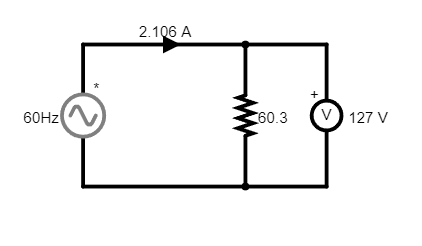
\includegraphics[width=0.5\textwidth]{figuras/circ-rede-falstad.png}}
    \fonte{}
\end{figure}

\begin{figure}[htb!]
    \caption{\textit{Setup} básico para testes completo.}
    \label{fig:setup-main2}
    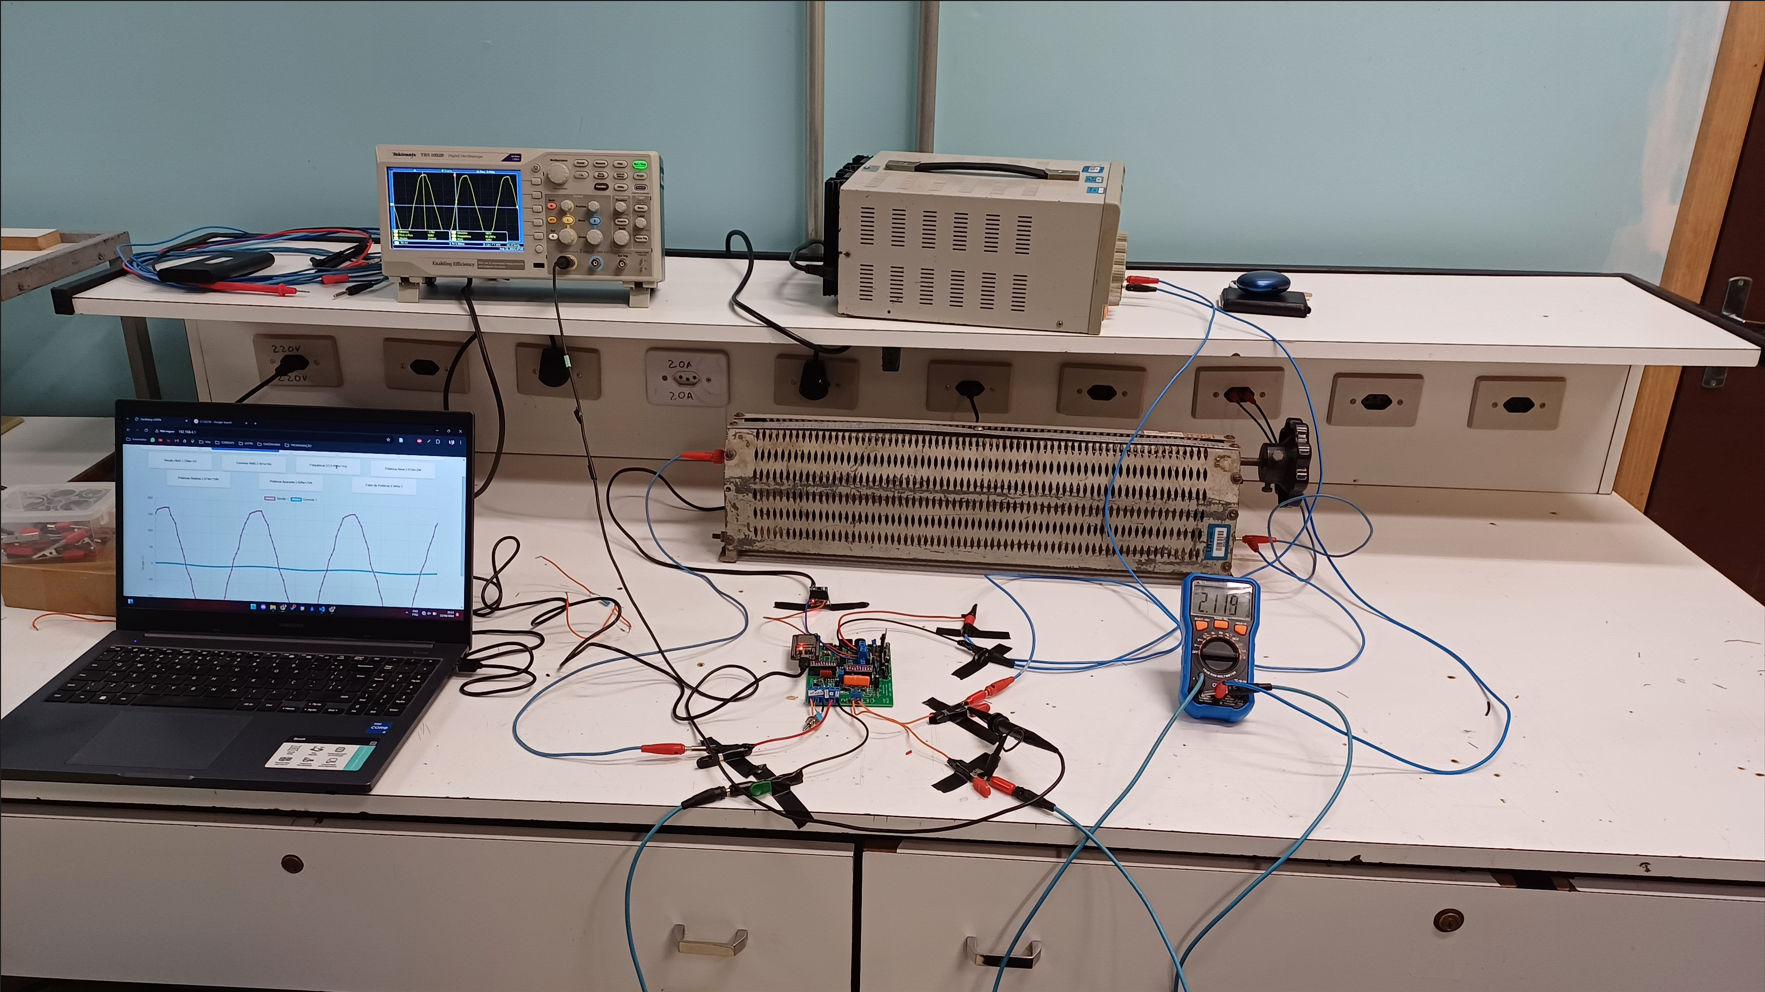
\includegraphics[width=0.8\textwidth]{figuras/setup-basico-full.png}
    \fonte{}
\end{figure}

Os resultados das medidas obtidos se encontram na tabela \autoref{tab:resultados-01} e as formas de onda nas Figuras \ref{fig:leitura-rede-osc} e \ref{fig:leitura-rede-boy-ondas}, obtidos pelo osciloscópio e o protótipo respectivamente. 

Além disso, também é possível observar os dados de frequência da rede, as potências ativa, reativa, aparente e o fator de potência, obtidos pelo protótipo.

\begin{figure}[htb!]
    \caption{Leitura da tensão do circuito do teste de leitura de rede - Osciloscópio.}
    \label{fig:leitura-rede-osc}
    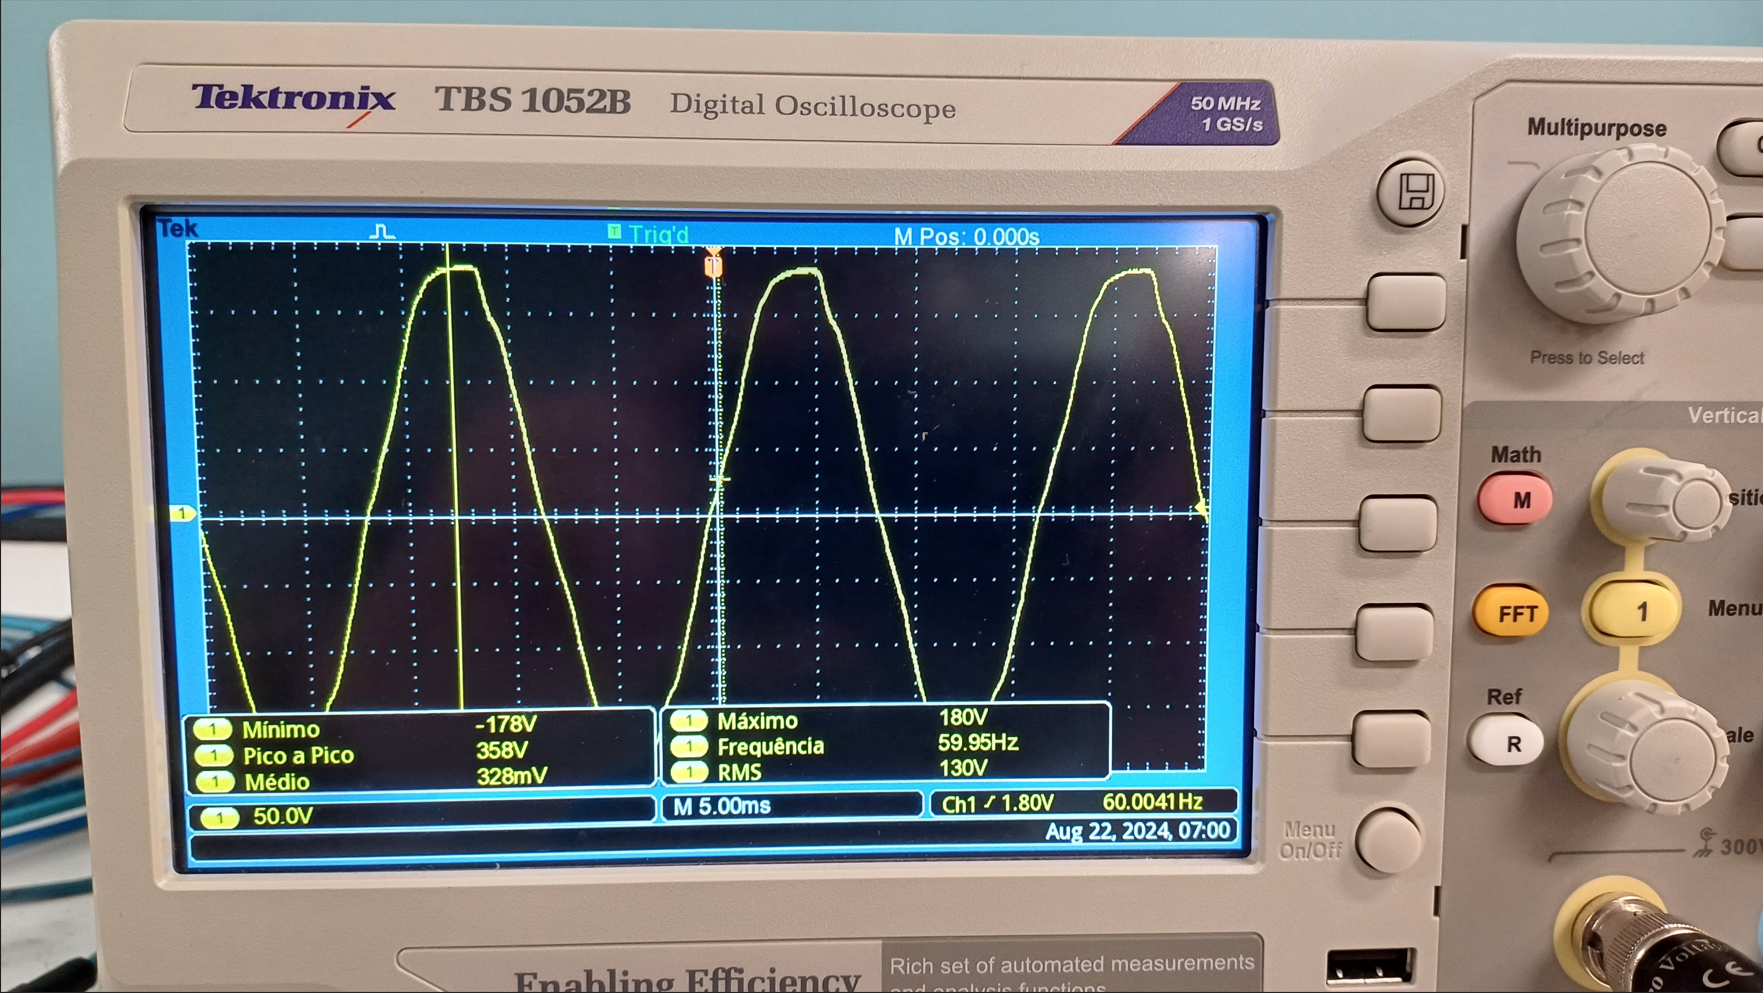
\includegraphics[width=0.8\textwidth]{figuras/leitura-rede-osc.png}
    \fonte{}
\end{figure}

\begin{figure}[htb!]
    \caption{Leitura completa do circuito do teste de leitura de rede - Protótipo}
    \label{fig:leitura-rede-boy-ondas}
    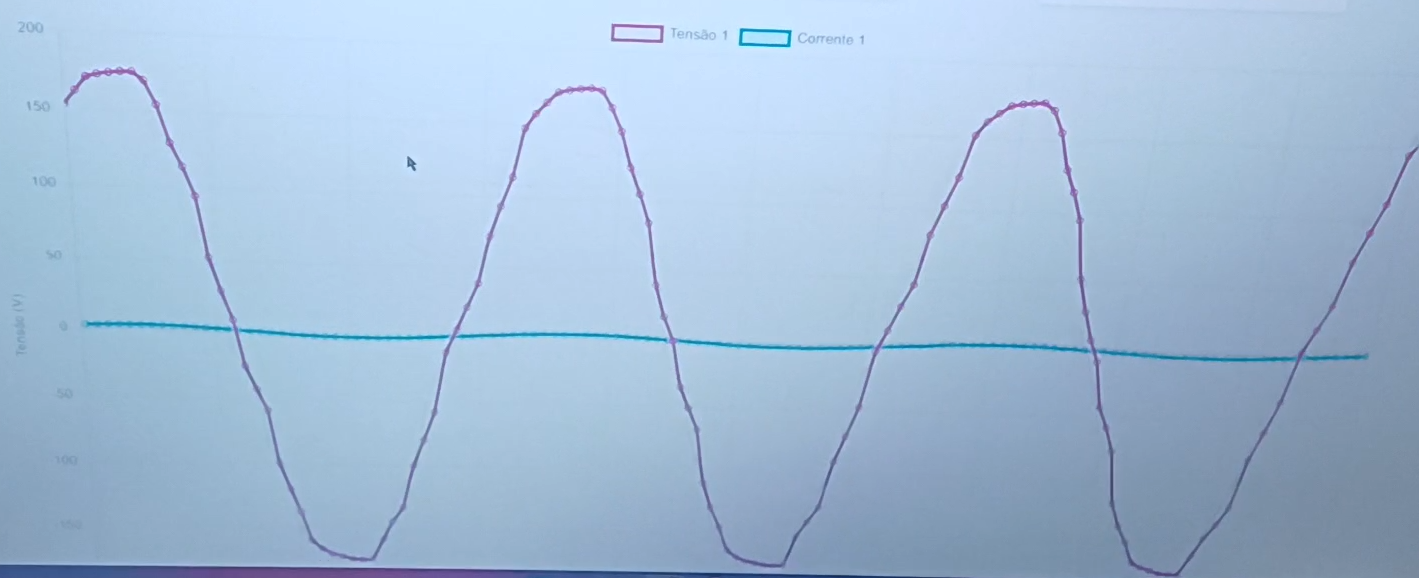
\includegraphics[width=0.8\textwidth]{figuras/leitura-rede-boy-ondas.png}
    \fonte{}
\end{figure}

Comparando os sinais obtidos, percebe-se que o protótipo propõe uma qualidade de leitura excepcional para este range. A tabela \autoref{tab:resultados-01} contém os resultados e também o erro do protótipo considerando os valores do osciloscópio (erro 1) e do multímetro (erro 2) como referência.

\begin{table}[!ht]
    \centering
    \caption{Resultados do teste de leitura da rede.}
    \label{tab:resultados-01}
    \begin{tabular}{ l l l l l l }
        \hline
        \textbf{Leitura} & \textbf{Osciloscópio} & \textbf{Multímetro} & \textbf{Protótipo}  & \textbf{Erro 1}  & \textbf{Erro 2}  \\ \hline
        Rede (V)         & 130 V                 & 128,7 V             & 128,1 V             & 1,46\%           & 0,47\%           \\ 
        Rede (A)         & -                     & 2,129 A             & 2,130 A             & -                & 0,047\%          \\ \hline
    \end{tabular}
    \fonte{}
\end{table}



\section{Teste 200 mVp}\label{teste-200mv}

O segundo teste propõe a verificação de outro range de leitura do protótipo. Para isto, um sinal de 200 mV pico foi gerado por um gerador de funções, conforme a \autoref{fig:ger-func-200}. Nota-se que na tela do gerador de funções se encontra a nomenclatura "Vpp", ou tensão de pico a pico, porém esta está equivocada, como demonstrado nos resultados das medições tanto do osciloscópio quanto do protótipo.

\begin{figure}[htb!]
    \caption{Gerador de funções - Sinal 200 mVp.}
    \label{fig:ger-func-200}
    \includegraphics[width=0.8\textwidth]{figuras/ger-func-200.png}
    \fonte{}
\end{figure}

\begin{figure}[htb!]
    \caption{Diagrama do circuito do teste de 200 mVp}
    \label{fig:circ-200}
    \fbox{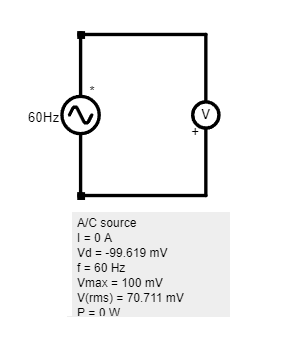
\includegraphics[width=0.5\textwidth]{figuras/circ-200-falstad.png}}
    \fonte{}
\end{figure}

Utilizando-se novamente o osciloscópio e um multímetro, obtém-se os valores de leituras indicados na \autoref{tab:resultadoss-200}. As Figuras \ref{fig:leitura-200-osc} e \autoref{fig:leitura-200-boy-onda} representam também um comparativo das ondas obtidas.

\begin{figure}[htb!]
    \caption{Leitura da onda de 200 mVp - Osciloscópio}
    \label{fig:leitura-200-osc}
    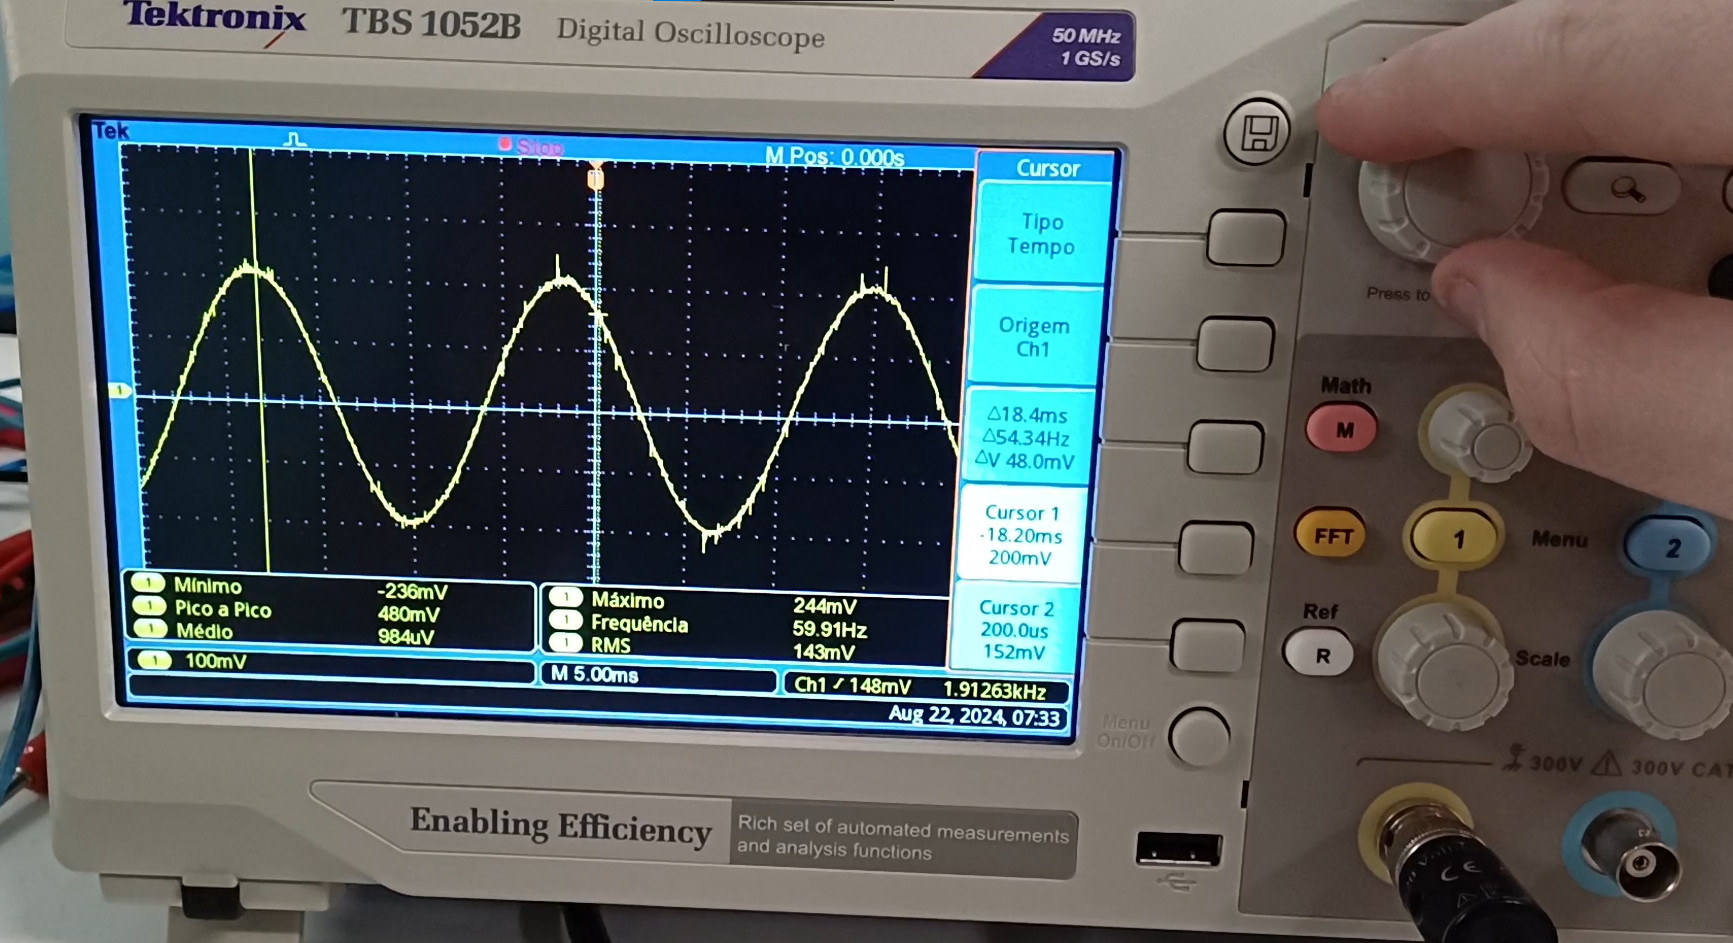
\includegraphics[width=0.8\textwidth]{figuras/leitura-200-osc.png}
    \fonte{}
\end{figure}

\begin{figure}[htb!]
    \caption{Leitura da onda de 200 mVp - Protótipo}
    \label{fig:leitura-200-boy-onda}
    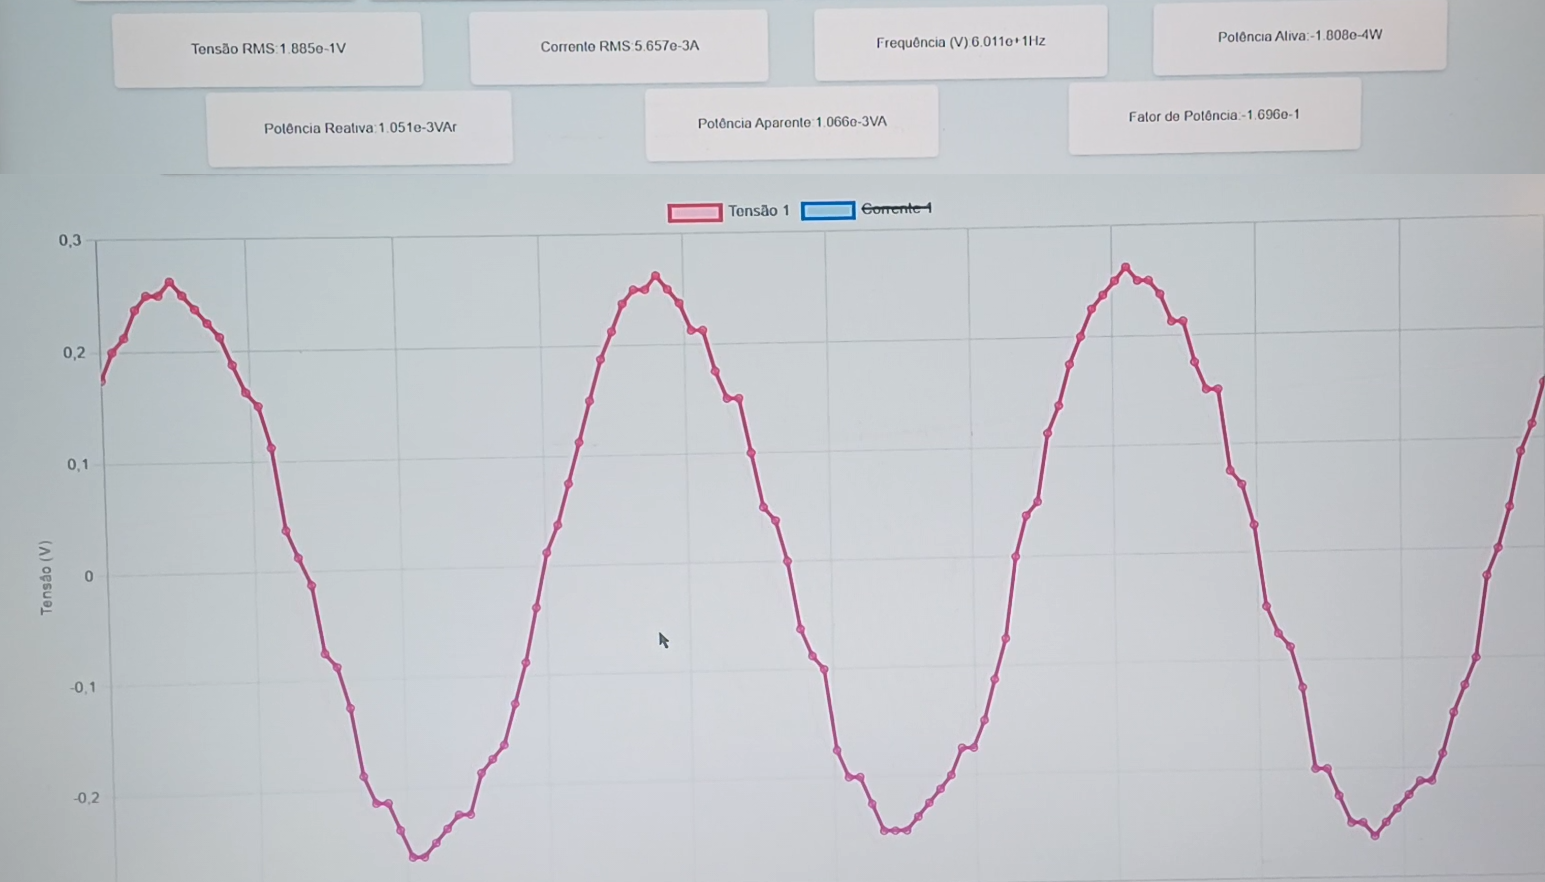
\includegraphics[width=0.8\textwidth]{figuras/leitura-200-boy-onda.png}
    \fonte{}
\end{figure}

\begin{table}[!ht]
    \centering
    \caption{Resultados do teste de 200 mVp.}
    \label{tab:resultadoss-200}
    \begin{tabular}{ p{2cm} p{3cm} p{2cm} p{2cm} p{2cm} p{2cm} }
        \hline
        \textbf{Leitura} & \textbf{Osciloscópio} & \textbf{Multímetro} & \textbf{Protótipo}    & \textbf{Erro 1}  & \textbf{Erro 2}   \\ \hline
        200 mVp          & 143 mVRMS / 244 mVp   & 137 mVRMS           & 188 mVRMS / 263 mVp   & 31,47\% e 7,78\% & 37,23\%           \\ \hline
    \end{tabular}
    \fonte{}
\end{table}

Comparando os sinais obtidos, a diferença entre todos os diferentes instrumentos é notável neste range de leitura. O protótipo apresenta um erro fora do proposto pelas espeficicações. Este range pode ser melhor calibrado por software e seu erro curado a ponto de respeitar tais especificações. Nota-se também que existem valores de corrente e potências, porém o canal de tais não está conectado, sendo estes então descartáveis.

\section{Teste uA}\label{teste-ua}

Para o range de leitura de corrente de micro amperes, foi utilizado um resistor comum de 30 k$\Omega$, sendo o valor real do resistor utilizado 32,63 k$\Omega$. Além disto, utilizou-se o gerador de função novamente para gerar uma tensão pequena de 10 Vp ou 7.07 V. Com estes dados, utilizando novamente a lei de Ohm, se espera uma leitura de corrente de 0,000217 A ou 217 $\mu$A.

\begin{figure}[htb!]
    \caption{Diagrama do circuito do teste de $\mu$A}
    \label{fig:circ-ua}
    \fbox{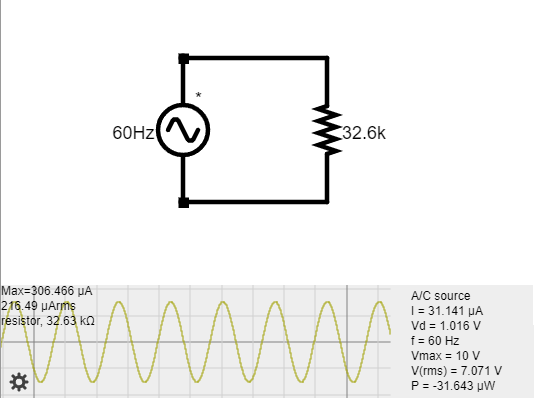
\includegraphics[width=0.5\textwidth]{figuras/circ-ua-falstad.png}}
    \fonte{}
\end{figure}

As leituras obtidas pelo multímetro e pelo protótipo são demonstradas na tabela \autoref{tab:resultados-ua} e as formas de onda na \autoref{fig:leitura-micro-boy-onda}.

\begin{figure}[htb!]
    \caption{Leitura da corrente de 217 $\mu$A - Protótipo.}
    \label{fig:leitura-micro-boy-onda}
    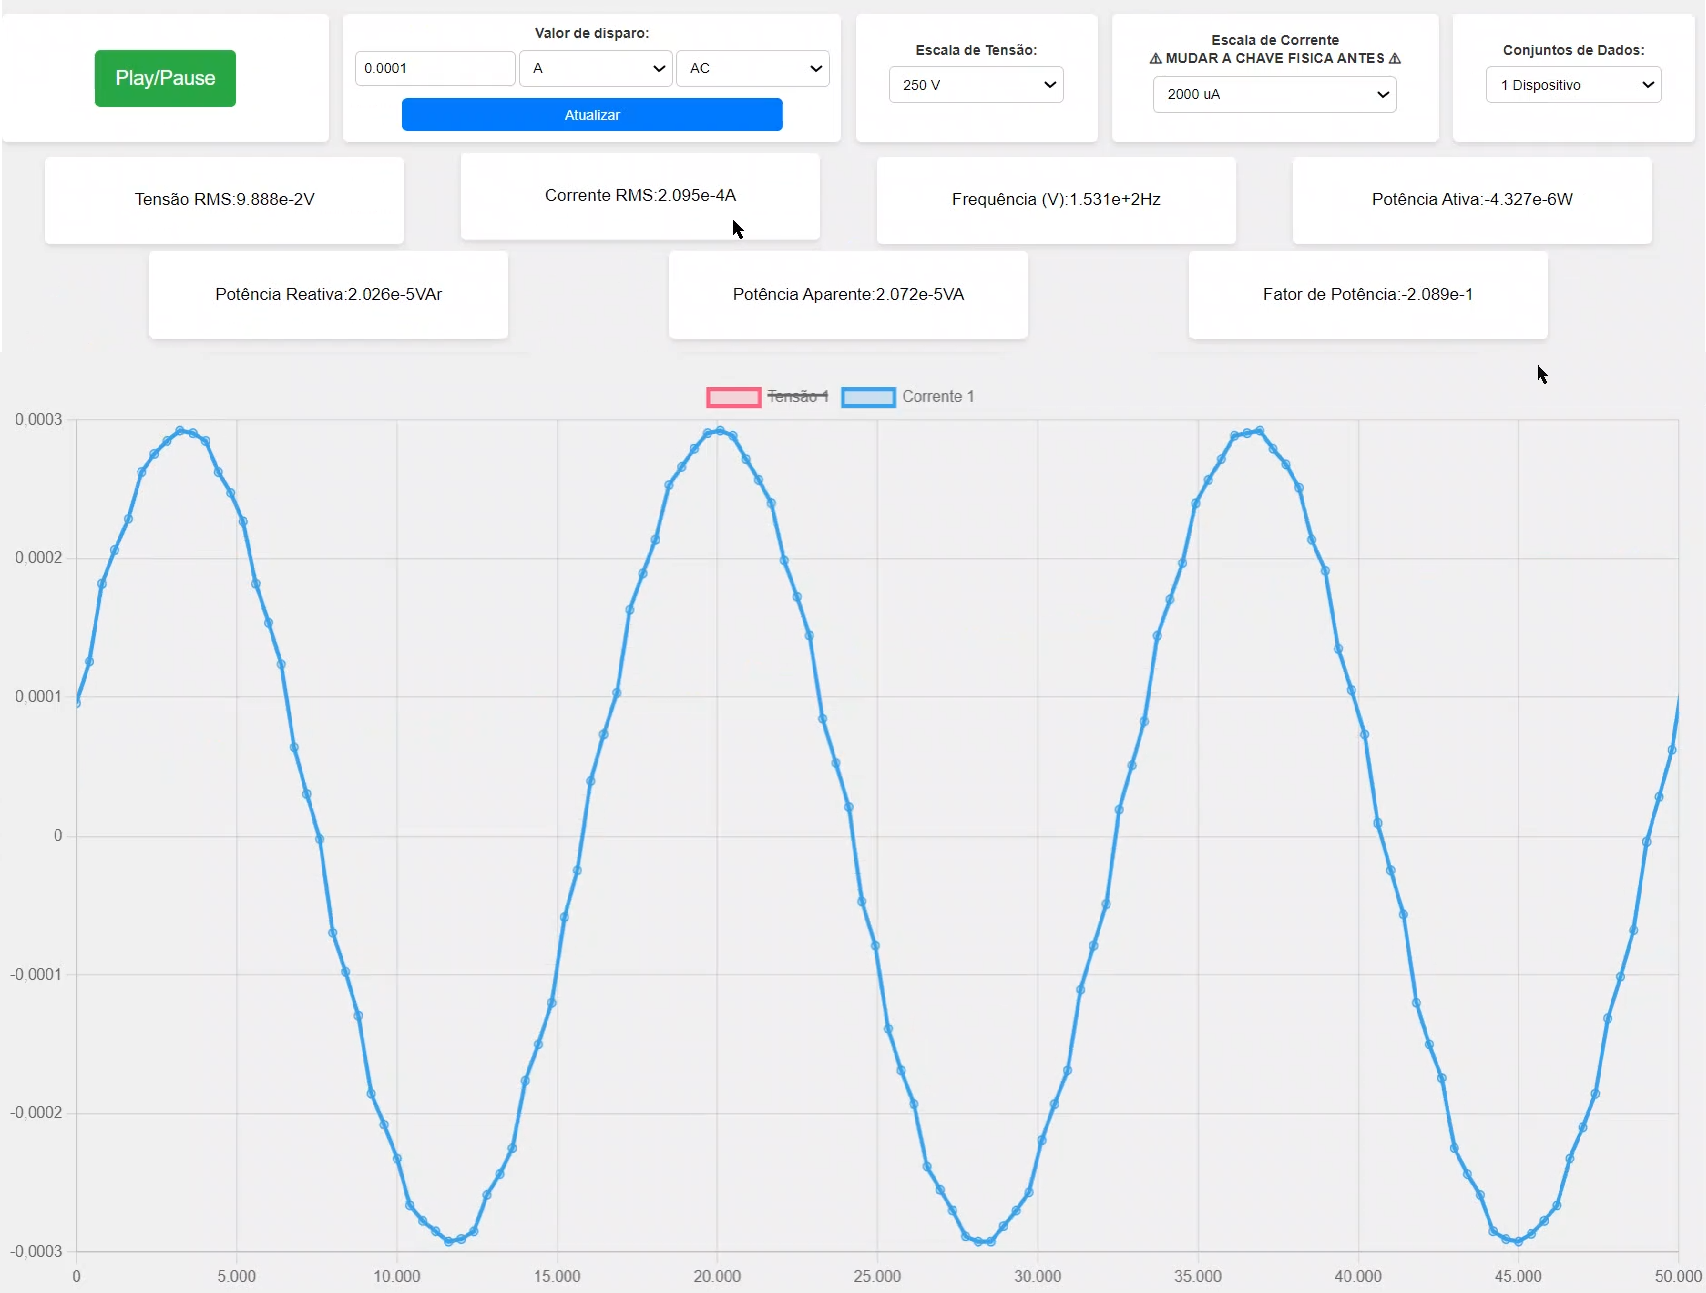
\includegraphics[width=0.8\textwidth]{figuras/leitura-micro-boy-onda.png}
    \fonte{}
\end{figure}

Olhando para os valores obtidos, percebe-se que tanto o multímetro quanto o protótipo exibem leituras precisas, confirmando assim a capacidade deste de ler sinais relativamente pequenos em ordem de magnitude.

\begin{table}[!ht]
    \centering
    \caption{Resultados do teste de $\mu$A.}
    \label{tab:resultados-ua}
    \begin{tabular}{ l l l l }
        \hline
        \textbf{Leitura}  & \textbf{Multímetro}  & \textbf{Protótipo}  & \textbf{Erro}   \\ \hline
        217 $\mu$A        & 214.9 $\mu$A         & 209.5 $\mu$A        & 2,51\%             \\ \hline
    \end{tabular}
    \fonte{}
\end{table}

\section{Teste \textit{Wheatstone}}\label{teste-Wheatstone}

Para provar a capacidade tanto de leitura DC quanto de leitura de tensão e corrente em pontos diferentes do circuito, foi utilizado um circuito de Wheatstone. Foram feitas as medições de acordo com o diagrama representado pela \autoref{fig:diagrama-circ-wheatstone} e sua montagem na \autoref{fig:circuito-wheatstone-full}. Como indicado no diagrama do circuito, são esperadas leituras de 3,75 V e 16,25 mA.

\begin{figure}[htb!]
    \caption{Diagrama circuito \textit{Wheatstone}}
    \label{fig:diagrama-circ-wheatstone}
    \fbox{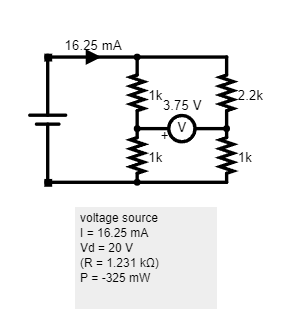
\includegraphics[width=0.8\textwidth]{figuras/diagrama-circ-wheatstone.png}}
    \fonte{}
\end{figure}

\begin{figure}[htb!]
    \caption{Circuito \textit{wheatstone}}
    \label{fig:circuito-wheatstone-full}
    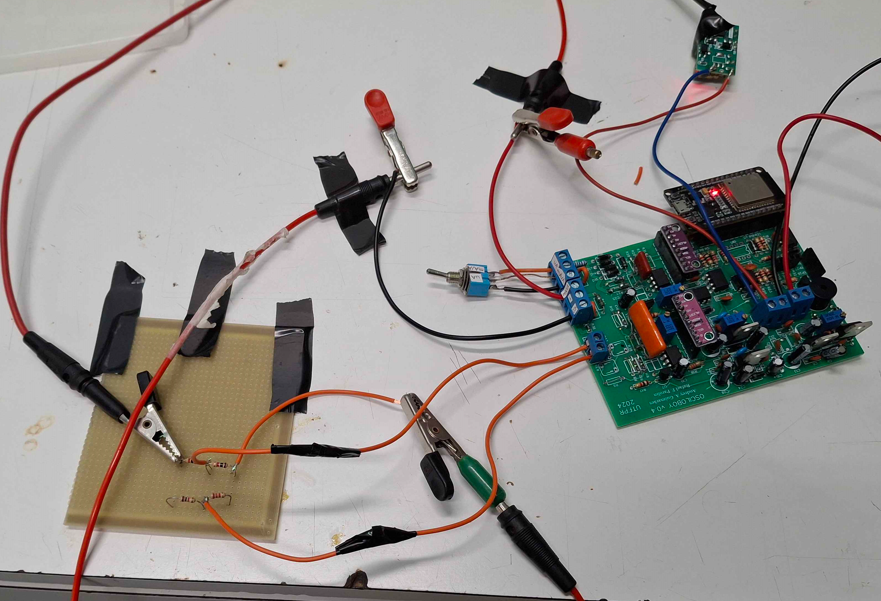
\includegraphics[width=0.8\textwidth]{figuras/circuito-wheatstone-full.png}
    \fonte{}
\end{figure}

A resistência equivalente deste circuito, quando medida, resultou em 1,21 k$\Omega$. As medidas obtidas estão representadas na \autoref{tab:resultados-wheatstone} e as formas de onda obtidas pelo osciloscópio e pelo protótipo nas Figuras \ref{fig:wheatstone-osc} e \ref{fig:wheatstone-boy}, respectivamente.

\begin{figure}[htb!]
    \caption{Leitura de tensão do circuito \textit{Wheatstone} - Osciloscópio}
    \label{fig:wheatstone-osc}
    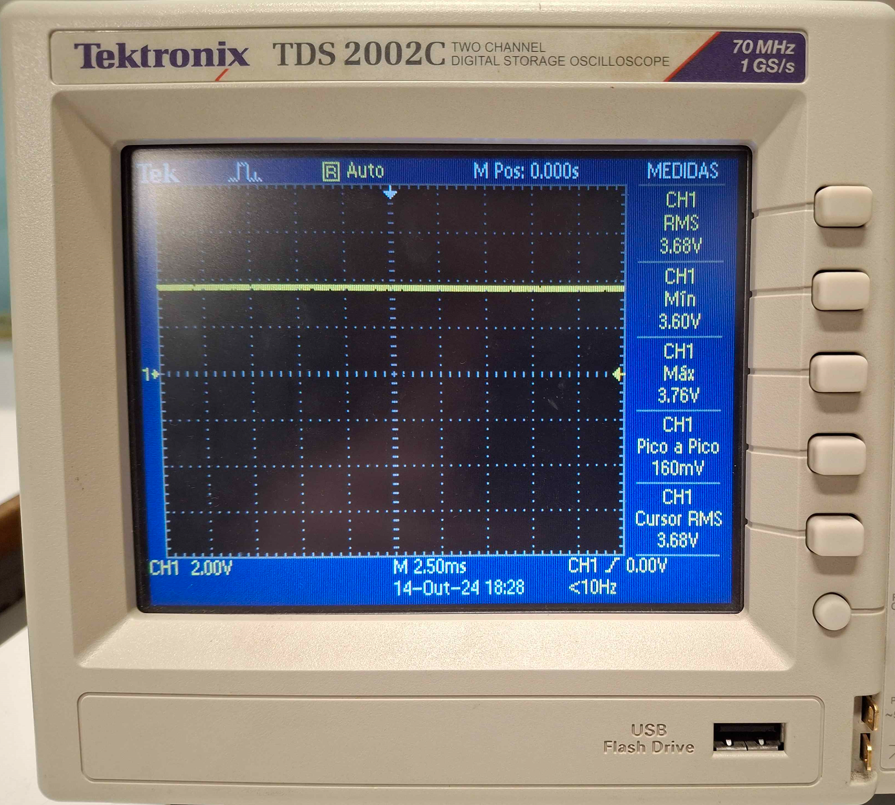
\includegraphics[width=0.8\textwidth]{figuras/wheatstone-osc.png}
    \fonte{}
\end{figure}

\begin{figure}[htb!]
    \caption{Leitura do circuito \textit{Wheatstone} - Protótipo}
    \label{fig:wheatstone-boy}
    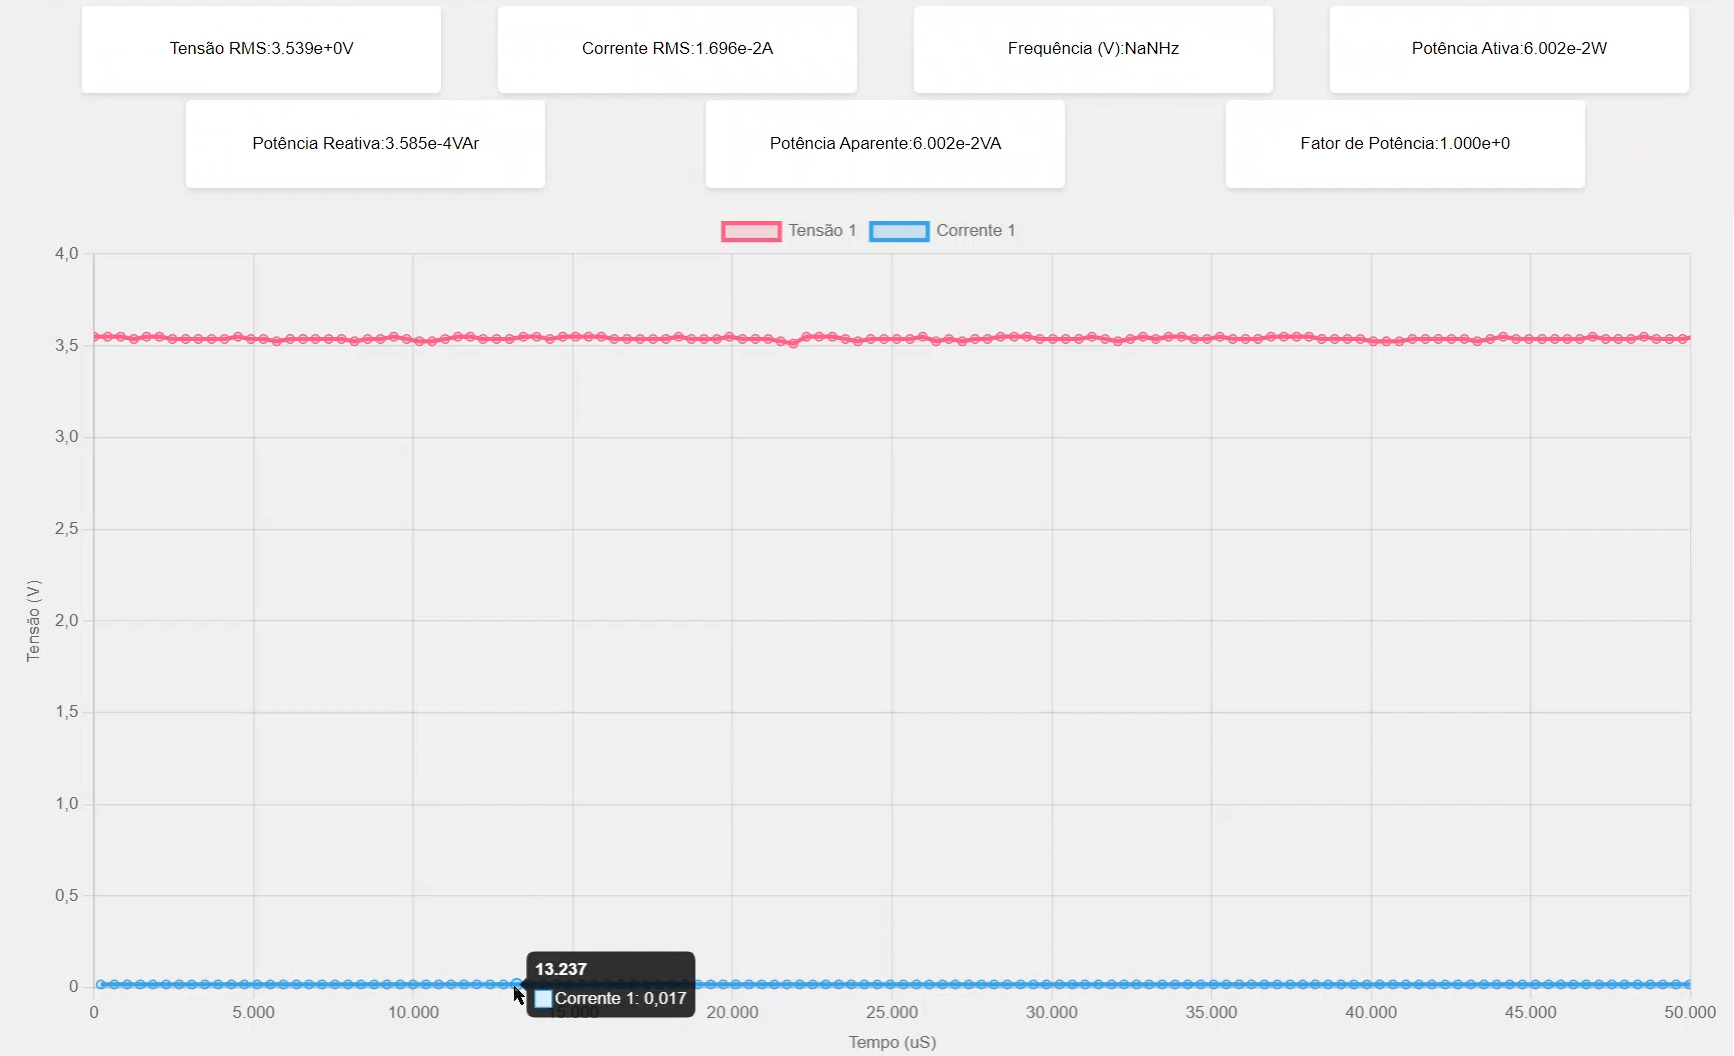
\includegraphics[width=1\textwidth]{figuras/wheatstone-boy.png}
    \fonte{}
\end{figure}

Comparando os resultados obtidos, é possível observar que as leituras de sinais de corrente contínua feitas pelo protótipo são de boa qualidade. Além disso, observa-se que este realmente possui a capacidade de leitura em pontos diferentes do circuito sem interferências ou erros.

\begin{table}[!ht]
    \centering
    \caption{Resultados do teste do circuito \textit{Wheatstone}.}
    \label{tab:resultados-wheatstone}
    \begin{tabular}{ l l l l l l }
        \hline
        \textbf{Leitura} & \textbf{Osciloscópio} & \textbf{Multímetro} & \textbf{Protótipo}    & \textbf{Erro 1}  & \textbf{Erro 2}   \\ \hline
        3,75 V           & 3,68 V                & 3,67 V              & 3,54 V                & 3,8\%            & 3,54\%            \\ 
        16,25 mA         & -                     & 16,51 mA            & 16,96 mA              & -                & 2.72\%            \\ \hline
    \end{tabular}
    \fonte{}
\end{table}